\chapter{Stock market data}

The aim of this chapter is to introduce a set of variables related to the financial market, 
their possible importance in terms of predictive modelling, and lastly their subsequent processing 
into specific forms, which were used throughout all the related analyses in this thesis.
\par
Market itself and particularly the price movement of financial instruments is a complex and unsurprisingly
counterintuitive process with a large number of various related variables, which contribute to price movements. 
In terms of using such data as an auxiliary source for decision making in investment strategy creation, there is a rich
universe of sources dealing with the issue \cite{clanok1, clanok2}.
\par
%
In the thesis, we aim mainly to research the predictive power of various diversely sophisticated
methods of machine learning on the particular market segment. Many papers tend to focus on a
single stock or a very limited set of a few stocks \cite{clanok5, konferencia1}. Others tend to apply predictive modelling methods
to stock indices (e.g. US S\&P 500 and NASDAQ Composite or German DAX) \cite{clanok4} however, there is 
a small number of sources dealing with a market segment, analyzing single stocks included in it.
\par
Our main focus is on the index S\&P 500 – a US stock index accumulating the 500 biggest publicly traded companies
in terms of market capitalization. The index itself is considered to be the most trustworthy general indicator of the overall
US and world’s stock economy state \cite{snp500}. The index itself is divided into several general market segments to which stocks belong. In this
thesis, we focused on the segment \textbf{Information technology}. However, the approach used in our analyses is adaptable to any subset of stocks –
the only determining constraint is the respective database of stocks.
\par
As of late 2025, the Information technology (IT) segment consists of $68$ US-traded stocks. However, we excluded three stocks, as their brief period of trading yielded insufficient historical data for reliable modeling. In the year 2025, in terms of total capitalization, the IT group makes a total of
nearly 30 \% of the index, which makes it the most weighted sector, despite making only 13.6 \% of all included stocks \cite{cnbc}. This recent growth of its weight 
could be explained by a lot of factors steering the market nowadays, but the general view on the topic suggests that recent boom of artificial 
intelligence could be the most dominant engine of growth. This suggests that focusing on this segment is reasonable, as it could be considered the most important one nowadays.

\section{Variables in financial data}
At first, we introduce specific attributes which define the value movement of all financial and economic instruments used throughout the thesis 
as features and target variables. These attributes could be further generalized onto any financial instrument attribute's movement, not only to price 
itself – as it will be applied to non-stock data as well.
\par
For the purposes of defining desired terminology, let's define a time interval on which we analyse an instrument's attribute movement as $[t_1, t_2]$, where
naturally $t_1 < t_2$. Defined attributes, which are attached to a single time breakpoints, could be universally defined for any time interval with various frequency.
\par
At the breakpoint $t_1$ we define the \textbf{opening value}, which denotes the value of the attribute at the very beginning of the interval. For the purposes of this thesis,
where we aim to use a daily frequency of data, this value denotes the value of the attribute at the very start of the trading day. In the opposite manner, at the breakpoint $t_2$ we define the 
\textbf{closing value}, denoting the final value of the attribute at the end of the observed interval – in our case, at the end of the trading day.
\par
During the process of value evolving throughout the interval, we observe the global minimum and maximum of the attribute's value, which we denote \textbf{low value} and \textbf{high value}, respectively.
Such data give us an indication of volatility during the interval and subsequently the sentiment of the market regarding the attribute.

The visualisation of the terms for a sample interval of a Microsoft stock between the beginning of June 2025 and the beginning of September 2025 is pictured in Figure \ref{fig:2.1}.
\par
Last but not least, we accumulate data regarding the number of an instrument's stocks traded (either sold or bought) during the time interval. This is denoted as \textbf{volume}, and in terms of
the thesis, the value of this attribute is known for stocks only; for other instruments we use the value of zero.
\par
The last data attribute, applied only on stocks' data as well, is volume of \textbf{dividends} paid out. Certain companies oblige themselves
to pay parts of their profit to their investors on a regular basis (e.g., Apple, Microsoft or Oracle) \cite{dividendy}. Some companies do not pay out dividends, even though this attribute was included in the database for all included stocks.
\begin{figure}[H]
    \centering
    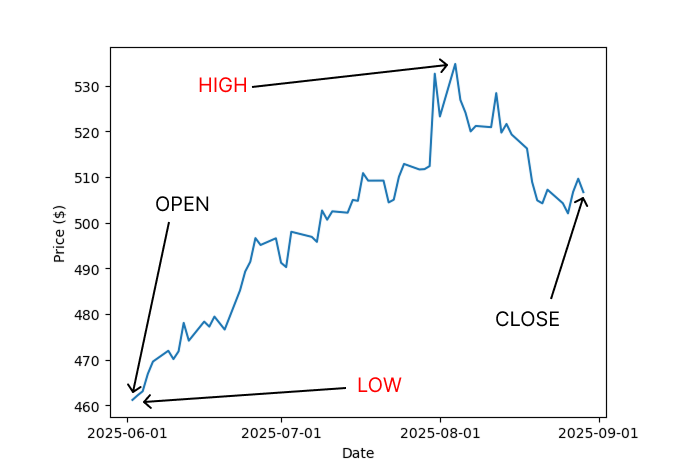
\includegraphics[width=0.9\linewidth]{images/TermsVisual.png}
    \caption{\centering Visualisation of the defined attribute's movement terms on Microsoft stock price.}
    \label{fig:2.1}
\end{figure}
\section{Rolling window and prediction methodology}
\label{rolling}
There are several approaches for splitting time-series data into training, validation, and test sets. For the purposes of next-day prediction — where data from trading days $t-q, t-(q-1), \dots, t-1$ 
(for some $q$) are used to predict the closing price on day $t$ — the concepts of rolling window methodology are adopted \cite{forecast_book}.
\par
In our approach, we define a static time-series interval, which serves as a hybrid train-validation time interval. Let's define the overall data interval being between
$T_1$ and $T_2$ timepoints (let $T_2-T_1=M$). On this interval reside two frames of variables. 

Multivariate $\mathbf{X} \in \mathbb{R}^{M \times F}$, where $F$ denotes the number of features used, which serves 
as an input variable. Included features in $\mathbf{X}$ are values of selected financial variables, shifted backwards up to $q=9$ days. This means, that 
$\mathbf{X}[t]$ (the $t$-th row of $\mathbf{X}$) represents data available through days $t-1, t-2, \ldots, t-9$. \footnote{We chose the value of $q$ due to few reasons constant. Firstly, variable $q$ 
would result in larger time-complexity and necessity to optimize new parameter further. Secondly, we want to emphasize short-term market dynamics,
which are commonly observed in financial time series and documented in the literature \cite{forecast_book}.} 

Second, univariate $Y \in \mathbb{R}^M$ accumulates values of the target variable (next closing price) to the respective rows of $\mathbf{X}$. This means, that $Y[t]$ (the $t$-th value in the $Y$) is the value of the closing price on day $t$.
\par
Further, we define parameter $1 \leq p<M$, which is the length of the training subwindow, meaning how many \textit{next-day} predictions model would be trained on,
and $w$, which denotes the forecasting horizon, i.e., the number of time units into the future for which predictions are made. For the purposes of this thesis and its next-day prediction methodology we define $w=1$.

With respect to the adopted methodology, we can generalize the process of train and validation sets split, by creating a pseudocode demonstrating the relationship
between input and target matrices. Algorithm \ref{alg:sliding_window} shows what parts of the global $\mathbf{X}, Y$ are directly available at the certain moment of model building.
\begin{algorithm}[H]
\caption{Rolling-window on $(T_1, T_2)$ interval}
\label{alg:sliding_window}
\begin{algorithmic}
\State \# We assume $w \gets 1$
\State \# The prediction target day is $t+p+1$, we have available data up to day $t+p$
\State Set look-back window length $p$ 
\State Retrieve the feature variables' values into the $\mathbf{X}$
\For{each stock in database}
    \State Retrieve closing prices into the target $Y$
    \For{$t = T_1$ to $T_2 - (p + 1)$}
        \State $\mathbf{X}_{\text{train}} \gets \mathbf{X}[t : t+p]$  \>\>\>\>\>\>\> \# Z-score scaled
        \State $Y_{\text{train}} \gets Y[t : t+p]$
        \State $\mathbf{X}_{\text{predict}} \gets \mathbf{X}[t+p+1]$ 
        \State \# $\mathbf{X}_\text{predict}$ corresponds to the latest available data 
        \State Train model $\hat{f}$ on $(\mathbf{X}_{\text{train}}, Y_{\text{train}})$: so $\hat{Y}_{\text{train}}=\hat{f}(\mathbf{X}_{\text{train}})$ 
        \State Generate prediction: $\hat{f}(\mathbf{X}_{\text{predict}})$
    \EndFor
\EndFor
\end{algorithmic}
\end{algorithm}
\label{testing_sub}
From Algorithm \ref{alg:sliding_window} a few important properties of this method could be derived.
Firstly, respective intervals are overlapping and the shift between respective input and target matrices, at $t$ and $t+1$,
is a single time unit. Secondly, by allowing window overlapping, we maximize the number of possible training data points, 
making the training-validation process possibly more robust and general. Lastly, such setup would be implemented on train-validation interval $(T_1, T_2)$ and
on disjoint test interval likewise.

The multivariate $\mathbf{X}$ contains pre-chosen shifted variables (Subchapter \ref{subchapter:2.3}). In this thesis, time interval between September 15, 2017 and December 31, 2022 (1333 trading days)
is used as training-validation interval and time interval between January 1, 2023 and January 16, 2026 (761 trading days) is used as test interval.

At this point, it is appropriate to illustrate this data preparatory setup with a specific example in order to better understand Algorithm \ref{alg:sliding_window}.
Let $p=4$ and suppose we want to predict the closing price on January 20, 2022. We have complete data up to January 19, 2022. With fixed $q=9$ and given $p$
the available training and validation data points are depicted in Figure \ref{fig:2.3}. 
\begin{figure}[H]
    \centering
    
\includegraphics[width=1\linewidth]{images/rolling_example.png}
    \caption{\centering Sample algorithm step for predicting the closing price of a given stock on January 20, 2022, with $p=4$.}
    \label{fig:2.3}
\end{figure}
Such setup is iteratively being done for every single stock, both on train-validation and test intervals.

\section{Suitable features in modeling}
\label{subchapter:2.3}

The amount of variables, which are directly or indirectly generated together with 
day-to-day market running, is quite enormous, and one should consider subsetting them 
for machine learning purposes wisely. In this subchapter, we aim to show and justify the 
process of our general feature selection, mostly based on a priori knowledge of processes within
financial markets and the variables' most likely effect on stock markets.
\par
For the sake of completeness, data were obtained from the API directly fetching data
available on Yahoo Finance – available through the Python library abstraction provided by the \texttt{yfinance} library \cite{yfinance, yahoo}.

\subsection{Stock indices}

In order to process the current general state of the stock exchange we researched possibilities of
implementing data regarding the price development of certain stock indices. \textbf{Index} is an abstract 
concept of accumulating information regarding single stock assets into one unified asset, mostly using a predefined
weighted average of prices of the stocks included.
\par
The stock index is specifically designed to follow and replicate the performance of a given subset of stocks. Taking this into account,
by including such well-chosen indices, which copy a broader and more various scope of stocks on a given market, we may obtain valuable
information regarding the current state of the US market.
\par
For these purposes, we decided to include into our database two major stock indices. The general index \textbf{Standard's and Poor 500}, commonly
known as S\&P 500, is an index including the 500 biggest US-traded stocks based on total market capitalization. The index consists of a wide scope of various
segments making it robust and universal in terms of mirroring the overall US market state.
\par
Taking into account the scope of this thesis – the Information technology segment, we decided to include the index \textbf{NASDAQ Composite} (NASDAQ). The main
difference from S\&P 500 is its segment focus. NASDAQ focuses mainly on tech and IT companies, making it possibly a valuable piece of data for our database of feature data.  

\subsection{Commodities}

Commodities denote mainly raw resources and materials, which are traded mainly in uniform quality and large quantities. Their fundamental role in the market
comes from the fact that most of these assets play an essential part in further processing, consumption and industry. Matsumoto et al. suggest, that the commodity
market play a vital part in the whole financial segment, which suggests, that including such assets in the database might be sufficient \cite{clanok3}.
\par
For the purposes of this thesis, we included data regarding two major commodities – \textbf{crude oil} and \textbf{gold}. Even though there might not be a clear
connection to the IT sector, we believe that such data would bring valuable information about the general state 
of the whole global economy.
\par
Oil plays a vital role in keeping the world in motion, and a solid majority of the world's activities depend on its presence and availability.
This might imply that these dependencies on the global market would be projected into the price movement of the commodity.
\par
Last but not least, we introduce gold price movements into the database. For a wide range of reasons, gold still remains one of the most
prominent securities. Most modern currencies are dependent on a system, where gold acts as a security stabilizing currency movements and limiting
the governments issuing money. On top of that, governments rely on physical gold as a reserve in times of crises \cite{gold}. Taking these reasons into account, 
by including gold in the database of features, we assume we are obtaining valuable information regarding the world's economy state, crisis potential or investors' sentiment, etc.

\subsection{Currency pairs - FOREX}

Currency pairs and subsequently the \textbf{Foreign Exchange Market} (FOREX) denote a specific market, where the main traded goods are currencies. Traders involved in the market speculate 
on certain exchange pairs' volatility and bet on them in order to make a profit. The market itself determines
price of every possible currency pair, thus making the acquisition of certain amount of currency possible through various ways – currency $X$ could be
traded through currencies $Y$, $Z$, etc., making the market far more speculative than others. By the volume of instruments traded, this decentralized 
market is by far the largest market in the world \cite{forex1}.
\par
Being fully decentralized, meaning prices on this market are accepted worldwide, these data could be considered as a sufficient
indicator of currency relative strength and, by that, an indicator of a particular government's and economic competitivness of a certain country. Taking this into account,
we assume, that including such data inside our database would bring valuable information about the international competitivness of US economy towards other major economies 
and quantitative information about relations among major economies, which is most likely an important predictor for stock price movements.
\par
By our focus on the US market, we chose to include currency pairs with the American dollar (\textbf{USD}) in all pairs. We chose to include so-called \textbf{major currency pairs},
with respect to their overall traded volume on a daily basis, according to reports published by the \textbf{Bank for International Settlements} and to market conventions \cite{bis_report, forex1}.
\par
In particular, included pairs, together with the USD, are the Euro \textbf{(EUR/USD)}, Japanese yen \textbf{(JPY/USD)}, British pound sterling \textbf{(GBP/USD)}, Swiss franc \textbf{(USD/CHF)}, Australian dollar \textbf{(AUD/USD)}, Canadian dollar \textbf{(USD/CAD)}, and New Zealand dollar \textbf{(NZD/USD)}.

\subsection{Other market indicators}
Apart from the introduced indicators and the general assets' price movement data above, there is still a vast group of
possibly valuable features, which do not fit into the above-defined features' groups. 
\par 
In order to track the performance of the US economy more precisely, it is wise to include information regarding national debt as possible features. 
For this purpose, we included data about \textbf{US Treasury bonds}. Bonds denote a financial instrument mostly long-term, low-risk securities
issued by the government of the USA, where an investor, in basic terms, lends money to the government in exchange for periodic fixed payments.
These bonds are further divided based on their maturity – the time within which issuer obliges itself to fully repay issued money.
\par
Price movements of bonds with various maturities are considered to be a good indicator of the US economy, and thus of the stock market state \cite{clanok6}. In our database
of possible features we included bonds with a maturity of 13 weeks, which belong to the group of short terms bonds, and bonds with 5 year long maturity. This kind of maturity
is on the edge between long-term and medium-term. The choice reflects the need to track data regarding relatively very short horizon and a long one.
\par
Apart from the bond-related data we considered obtaining data which are not directly financial – they are not any type of asset. We researched possibilities of
tracking the sentiment of investors and of the market itself. We chose to include data of \textbf{Volatility Index} (VIX), which is a specific gauge tracking state
of the US stock market in terms of volatility and the sentiment of investors. 
\par
It presumably brings valuable information, which might not be included in all of the metrics described, regarding the a priori mood of the market 
and its assets' risk. Its value ranges mostly up to $80$, which was considered as crisis values in years $2020$ and $2008$, and above approximately $10$, which
is considered to be relatively stable market state. Value development between the January and September of 2025 is given in Figure \ref{fig:2.2}.

\begin{figure}[H]
    \centering
    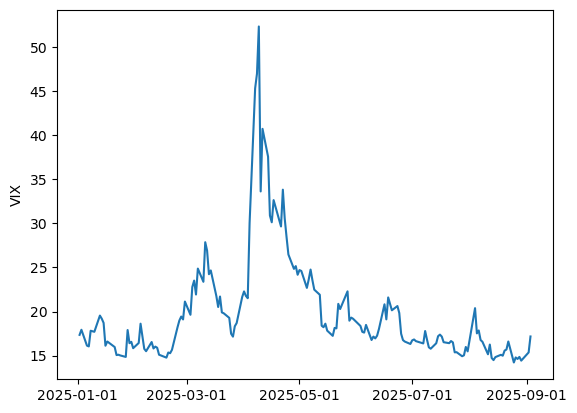
\includegraphics[width=0.7\linewidth]{images/VIX_example.png}
    \caption{\centering VIX value movement through the 2025.}
    \label{fig:2.2}
\end{figure}

It is surely interesting to address the sudden VIX surge during the April 2025. This sudden increase was basically day-to-day and denotes 
phase of repeated issuing and cancelling of international tarrifs. As we can see, this political move damaged investors' exposure to the US market then.